\documentclass[tikz,border=8pt]{standalone}
\usetikzlibrary{arrows.meta}
\begin{document}
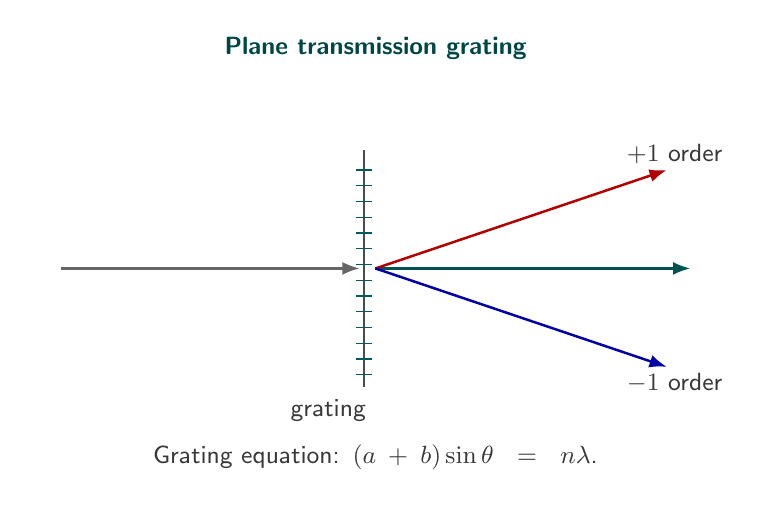
\begin{tikzpicture}[
  ray/.style={-{Latex[length=2.2mm]},line width=0.9pt},
  line/.style={draw=black!70,line width=0.75pt},
  label/.style={font=\sffamily\small,text=black!78},
  title/.style={font=\sffamily\bfseries\small,text=teal!55!black},
]
\node[title] at (0,2.8) {Plane transmission grating};
\draw[line] (-0.15,-1.5)--(-0.15,1.5);
\foreach \y in {-1.35,-1.15,...,1.35}{\draw[teal!70!black] (-0.25,\y)--(-0.05,\y);}
\draw[ray,draw=black!60] (-4,0)--(-0.2,0);
\draw[ray,draw=teal!65!black] (0,0)--(4,0);
\draw[ray,draw=red!70!black] (0,0)--(3.7,1.25);
\draw[ray,draw=blue!65!black] (0,0)--(3.7,-1.25);
\node[label] at (-0.6,-1.8) {grating};
\node[label] at (3.8,1.45) {$+1$ order};
\node[label] at (3.8,-1.45) {$-1$ order};
\node[label,align=center,text width=8.6cm] at (0,-2.4)
  {Grating equation: $(a+b)\sin\theta=n\lambda$.};
\end{tikzpicture}
\end{document}
